% Chapter 1
\makeatletter
\def\input@path{{../}}
\makeatother
\documentclass[../main.tex]{subfiles}
\begin{document}
\chapter{Introduction} % Chapter title

\label{ch:intro} % For referencing the chapter elsewhere, use \autoref{ch:introduction}

\section{Research problem exploration - literature review}

\subsection{Turbulence}
\begin{flushright}{\slshape}    
Finally, there is a physical problem that is common to many fields, that is very old, and that has not been solved. It is not the problem of finding new fundamental particles, but something left over from a long time ago—over a hundred years. Nobody in physics has really been able to analyze it mathematically satisfactorily in spite of its importance to the sister sciences. It is the analysis of circulating or turbulent fluids. \\ \medskip
--- \defcitealias{knuth:1974}{Donald E. Knuth}\citetalias{RichardFeynmann}\citep{Feynmann_I}
\end{flushright}

 Richard Feynmann said these words  more then 50 years ago  and his message seems to be still valid. Fluid turbulence has attracted the attention of physicists, mathematicians, and engineers for over one hundred years. Phenomenon of turbulence present in nature is mostly associated with the observational aspects, which play far more important role due to the unsatisfacory state of "theory": a theory based on first principles simply does not exist. There is no consensus about physical definition of "turbulent motion" or agreement on mathematical "turbulence problem" to be solved. However unlike other complicated physical phenomena it is easy to observe at least some of the numerous manifestations of turbulence. Major qualitative universal features of turbulent flow, that form the "essence" of turbulence, are listed below.

\begin{enumerate}
\item Spatio-temporal apparent randomness (chaoticity).\\
\item Extremely wide range of strongly and non-locally interacting degrees of freedom ($\sim 10^{18}-10^{29}$ in atmospheric flows \citep{Orlanski1975}), hence its extreme complexity enforcing statistical description.\\
\item Chaotic nature (manifest itself by loss of predictability of turbulent flows), which at the same time posses statistically stable properties.\\
\item Three dimensional and higly dissipative behaviour, thereby time irreversible and rotational. First two are probably the most specific and important attributes of turbulence.\\
\item Highly diffusive - turbulent flows exhibit strongly enhanced transport processes of momentum, energy and passive objects when compared to laminar flows.\\
\item Strongly nonlinear, non-integrable, nonlocal, non-Gaussian.
\end{enumerate}

The true turbulence theory should predict and explain universal properties listed above. The best we have so far is the set of equations developed almost 200 years ago, that describe fluid motion - Navier Stokes equations (NSE). Most probably it contains all of turbulence. The problem is that we do not know global solution of these equations, and the knowledge of specific solutions does not lead to understanding the dynamics or structure of turbulent processes as a whole.\\
\marginpar{Navier Stokes equations}
The Navier Stokes equation is a deterministic, nonlinear partial differential field equation. It can be presented in two ways that are used to describe the fluid motion. One is called Lagrangian, where one follows fluid particles along their trajectories. The other is called Eulerian, in which the observation of the system is made in a fixed frame as the fluid goes by. In Eurlerian formulation the NSE are as follows:
\begin{equation}
\overbrace{\underbrace{\frac{\mathrm{\partial}\vec{u}}{\mathrm{\partial}t}}_{(1)}+\underbrace{\vec{u}\cdot\nabla \vec{u}}_{(2)}}^{\frac{\mathrm{D}\vec{u}}{\mathrm{D}t}}=\underbrace{-\frac{1}{\rho} \nabla p}_{(3)} +\underbrace{\nu \nabla^2 \vec{u}}_{(4)}+\vec{f}
\label{ch1:eq01}
\end{equation}
where $\vec{u}$ - fluid velocity, $\rho$ - fluid density, $p$ - fluid static pressure, $\nu$ - kinematic viscosity, $\vec{f}$ - external forces.\\
Term (1) of NSE in this form is a standard partial time derivative. Term (2) represents advection of a fluid element. Those terms together create what is called the material derivative: $\frac{\mathrm{D}}{\mathrm{D}t}$. Term (3) expresses pressure gradient and term (4) represents viscous forces.\\
Dimensionless version of the NSE brings to life dimensionles quantity that is very important in fluid mechanics - the so-called Reynolds number $Re$. \marginpar{Reynolds number} It estimates the ratio of inertial forces (given by term (2) in \ref{ch1:eq01}) to viscous forces (given by term (4) in \ref{ch1:eq01}) within a fluid parcel. It can be presented with the use of characteristic scales of the fluid flow: $U$ - velocity scale and $L$ - length scale:
\begin{equation}
Re=\frac{UL}{\nu}
\label{def:Re}
\end{equation}
The primary physical interpretation of the Reynolds number is that for small $Re$ the flow is dominated by laminar motion and for large $Re$  the flow is mostly turbulent \citep{Reynolds1883}. The exact transition between these two regimes (at so called \emph{critical Reynolds number} $Re_{cr}$)\marginpar{critical Reynolds number} is specific for a geometry of the flow and has been a subject of separate, extensive studies. A quick estimation of the $Re$ number for a cumulus cloud, in which $L \sim$1~km, $U \sim$1~m/s, $\nu \sim10^{-5}$~$m^2/s$, leads to $Re \sim 10^8$ and the conclusion that the airflow in the cloud is extremely turbulent, since typical $Re_{cr}$ lays in in the range $10^2-10^6$.\\
\noindent Though NSE have a limited kinetic foundation, it is commonly believed to be \emph{adequate} i.e. its solutions corresponds to real fluid flows at all accessible $Re$, including turbulent flows. Unfortunately it is impossible to solve NSE analytically subject to most realistic initial and boundary conditions. For large Re the essence of the problem lies in the nonlinearity of the advection term (2) in Eq.\ref{ch1:eq01}.

\subsubsection{Phenomenology of turbulence}

Because a field theoretical solution of the Navier Stokes equation is elusive, the fruitful approach comes from asking questions concerning the physics of the processes. The problem is to identify, interpret and explain major fundamental physical mechanisms that result in the universal properties of turbulence. The first such comprehensive attempt to explain these mechanisms is phenomenological theory of cascade \citep{Richardson1922} enriched and quantified by Kolmogorov hypotheses \citep{Kolmogorov1941}. In the following, the foundations of these theories are outlined and the basic concepts commonly used in turbulence research are explained (description in this paragraph inspired by \citet{Pope2011} and \citet{Tsinober2001}).\\
Cascade concept postulates that in the flows of large $Re$ kinetic energy enters the turbulence through a production mechanism at the largest scales of the flow. This energy is then transferred by inviscid processes to smaller and smaller scales, until, at the smallest scales, the energy is dissipated by viscous action. \marginpar{TKE dissipation rate} This concept defines a rate of turbulent kinetick energy (TKE) dissipation $\epsilon$. \marginpar{eddy} The turbulent cascade scales emerge in the form of \emph{eddies} - moderately coherent structures of turbulent motion localized in the region of size constrained by the arbitrary scale.\\
Kolmogorov hypotheses state that for every turbulent flow, at sufficiently high Reynolds number, there exist scales $l_0$, $l_{EI}$, $\eta$ such that:
\begin{itemize}
\item small-scale turbulent motions $l<<l_0$ are statistically isotropic
\marginpar{local isotropy hypothesis}
\item the statistics of the small-scale motions $l<<l_{EI}$ have a universal form that is uniquely determined by $\nu$ and $\epsilon$
\marginpar{1st similarity hypothesis}
\item the statistics of the motions of scale $l$ in the range $\eta<<l<<l_0$ have a universal form that is uniquely determined by $\epsilon$, independent of $\nu$ \marginpar{2nd similarity hypothesis}
\end{itemize}

\begin{figure*}
\centering
\noindent 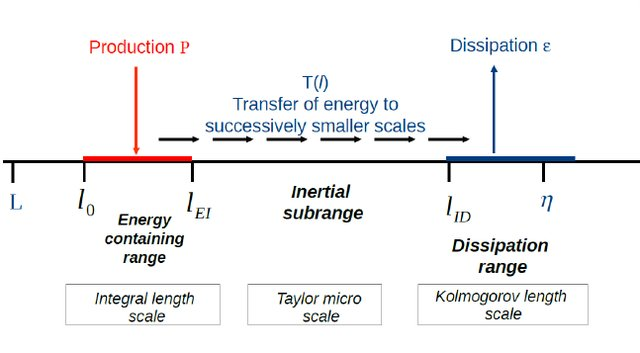
\includegraphics[width=30pc]{gfx/Turb_lenthscales_Pope.jpg}
\caption{Turbulent eddy size ranges and transfer of energy diagram ( from \citet{Saeedipour2014}).}
\label{fig:ch1_01}
\end{figure*}

Those hypotheses lead to a paradigmatic decomposition of the multiscale turbulence phenomenon to a few eddy size ranges illustrated schematically in the Fig. \ref{fig:ch1_01}. The scales are ordered as follows: $L>l_0>l_{EI}>\lambda>l_{ID}>\epsilon$. $L$ is the flow scale. $l_0$ is the scale of the smallest anisotropic eddies affected by the boundary conditions of the flow and $l_0$ is comparable to $L$. $l_{EI} $ demarcates between anisotropic eddies and smaller isotropic eddies of universal character. \marginpar{energy containing range}The range $[l_0, l_{EI}]$ is called \emph{energy containing range} and have bulk of the energy production. \marginpar{inertial range} \emph{Inertial range} $[l_{EI},l_{ID}]$, which is the name of the subrange described by 2nd similarity hypothesis, is governed only by inertial effects, viscous effects being negligible. \marginpar{dissipation range} The smallest scales, so called \emph{dissipation range}, are described by 1st similarity hypothesis. Based on scaling argument, out of its only parameters $\epsilon$ and $\nu$, Kolmogorov formed unique length, velocity and time scales for this range, which are now called Kolmogorov scales:
\marginpar{Kolmogorov scales}
\begin{align}
\eta \equiv (\nu^3/\epsilon)^{1/4} \sim Re^{-3/4} l_0\\
u_{\eta} \equiv (\epsilon \nu)^{1/4}\sim Re^{-1/4} u_0\\
\tau_{\eta} \equiv (\nu/\epsilon)^{1/2}\sim Re^{-1/2} \tau_0
\label{def:Kol_scales}
\end{align}
Reynolds number based on Kolmogorov scales is equal to one: $\frac{\eta u_{\eta}}{\nu}=1$. It is easy to see that the larger the $Re$ based on the flow scales, the greater is the span of scales in turbulent fluid.\\
\marginpar{Taylor microscale}
A well-defined quantity that is also often used in turbulence research (especially numerical simulations)  is the \emph{Taylor microscale} $\lambda$. It does not have a clear physical interpretation, but it is the intermediate length scale at which fluid viscosity significantly affects the dynamics of turbulent eddies in the flow. In Kolmogorov turbulence:
\begin{equation}
\lambda=\sqrt{15 \nu/\epsilon} \bar{u'}
\label{def:Tylor_scale}
\end{equation}
where $\bar{u'}$ is turbulence intensity - a root mean square of velocity fluctuations. Reynolds number built on this scale is called \emph{Taylor microscale Reynolds number} $Re_{\lambda}$.\\
Probably most important and commonly used conclusions from Kolmogorov's theory concern inertial range. Firstly there is the so-called \emph{"-5/3 law"}.\marginpar{-5/3 law} In the Fourier space formulation, this law concerns energy spectrum function $E(\kappa)$, which describes energy spectrum for the fluid velocity  Fourier modes of wavenumber $\kappa$ (here $\kappa$ is a scalar value). It states that in the inertial range the energy spectrum is a universal function of $\kappa$  and $\epsilon$ and is a power-law spectrum:
\begin{equation}
E(\kappa)=C \epsilon^{2/3} \kappa^{-5/3}.
\label{def:Ek_inertial}
\end{equation}
The constant $C$ is called Komogorov universal constant and experimental data support the value $C \approx 1.5$. Recent extensive DNS for example point to $C \approx 1.64$ \citet{Gotoh2002}. This law is often used in the structure function formulation as well. By the definition \emph{2nd order structure function} is a covariance of velocity difference between two points separated by $\vec{r}$: $\vec{x}+\vec{r}$ and $\vec{x}$:
\begin{equation}
D_{ij}(\vec{r},t)=\langle \left(u_i(\vec{x}+\vec{r},t)-u_i(\vec{x},t)\right)\left(u_j(\vec{x}+\vec{r},t)-u_j(\vec{x},t)\right)\rangle
\label{def:struct_fun}
\end{equation}
In locally isotropic turubulence $D_{ij}(\vec{r},t)$ is determined by a single scalar function, the longitudinal structure function $D_{LL}(r,t)$. And, according to similarity hypothesis, for large $r/\eta$ there is:
\begin{equation}
D_{LL}(r,t)=C_2 (\epsilon r)^{2/3},
\label{def:struct_fun_inertial}
\end{equation}
in the inertial range, where $C_2$ is a universal constant. $C_2 = \frac{72}{55} C \approx 2$. So that the energy spectrum "-5/3 law" corresponds to the "2/3 law" in the structure function formalism.\\
Figure \ref{fig:ch1_02} is a part of Fig. 5 and 6 in \citet{Jen-LaPlante2016}, a paper co-authored by the thesis author. It presents examples of power spectral density (PSD) and structure funtions calculated for one dimensional velocity data collected in the Stratocumulus (Sc) cloud top during TO10 flight of POST campaign. PSD refers to the spectral energy distribution, that would be found per unit time, since the total energy of such a signal over all time would generally be infinite. Sc cloud top was  split into several layers on the basis of turbulence, moisture and temperature field properties. Starting from the top of the top, FT is free troposphere, TISL - turbulent inversion sublayer, CTMSL - cloud top mixing sublayer and CTL is the cloud top layer.\\

\begin{figure*}
\centering
\noindent 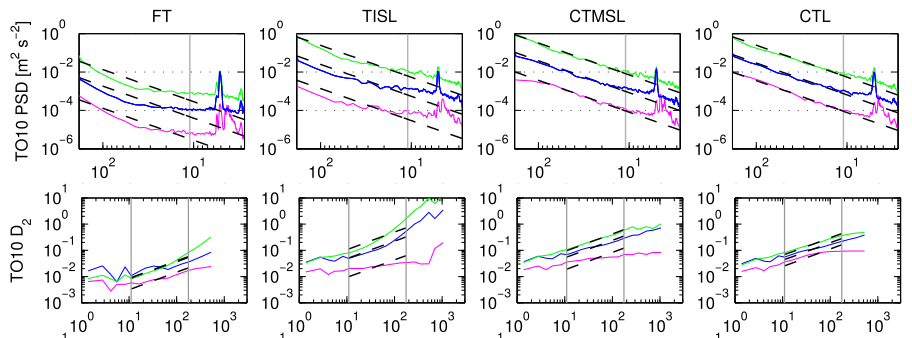
\includegraphics[width=30pc]{gfx/POST_spectra_struct.png}
\caption{Power spectral density ($PSD$) and 2nd order structure functions ($D_2$) of velocity fluctuations of the three components $u$, $v$, $w$ (blue, green, red) composites for all ascents/descents in single measurement flight (TO10) of POST campaign. Individual plots are shifted with respect to each other by factors of 10 for comparison, as indicated. Dashed lines show $-5/3$ slope for $PSD$ or $2/3$ slope for $D_2$ fitted in a range of frequencies from 0.3~Hz to 5~Hz, in order to avoid instrumental artifacts at higher frequencies. Each column heading corresponds to Sc cloud top sublayer of different properties: FT- free troposphere, TISL - turbulent inversion sublayer, CTMSL - cloud top mixing sublayer, CTL - cloud top layer.}
\label{fig:ch1_02}
\end{figure*}
The second theoretical model often used in data analysis is the "Taylor hypothesis" or "frozen-flow hypothesis" for inertial range. It says, that in the case of statistically stationary flow with turbulence intensity small compared to mean velocity, we can approximate spatial correlations by temporal correlations. Both the "-5/3 law" and Tylor hypothesis are commonly used to estimate $\epsilon$ from experimental data. This task is still however a matter of vivid discussion in cloud turbulence research \citep{Waclawczyk2017, Zilitinkevich2019}.\\
Kolmogorov's phenomenological theory is the only tool  developed so well that it can characterize turbulent flow in many diverse applications. It even constitutes the language of many different turbulence descriptions. Despite being a good approximation of tubulence phenomenon, experimental premises indicate that a large part of its basic assumptions is flawed and many mechanisms are not captured. There is evidence that anisotropy in large scales causes anisotropy of small scales and that there is coupling between large and small scales \citep{Warhaft2000}. The notion of "hierarchy" in turbulence is also doubted. Another important issue, not described by Kolmogorov's theory or its extensions, is the phenomenon of intermittency in small scales, inseparably connected with the notion of "structure" of turbulence. Intermittency and structure are the subject of the next paragraph.

\subsubsection{Structure of turbulence}

It is mostly agreed that turbulence posseses structure. It is agreed as well that some aspects of this structure are intimately related to \emph{intermittency}\marginpar{intermittency}. These topics have been addressed and detailed in the books by Arkady Tsinober \citep{Tsinober2001, Tsinober2014}. I summarised below some of the most important points.\\
Small-scale (or internal) intermittency is defined twofold: geometrically and statistically, and these aspects are not independent. The geometric definition refers to some examined quantity $x$. This quantity is intermittent when for any small value $x_0$, the volume of fluid in which $x>x_0$, decreases with increasing $Re$. In colloquial terms, when $Re$ increases, our examined value of x is more and more "spiky" in its domain. Statistically a variable $x$ with zero mean is intermittent if its probability distribution is such that extremally small and extremally large excursions are much more likely than in normally distributed variable (Gaussian).\\
Various experiments have shown that Lagrangian statistics in turbulent flows display Gaussianly distributed velocity values and non-Gaussianly distributed velocity differences or accelerations. Measured energy dissipation rate and vorticity are intermittent as well. Structures most probably responsible for the tails observed in the dissipative scales (sometimes referred to as \emph{extreme events}) are predominantly in the form of vortex tubes and strain sheets. \marginpar{vortex tubes}Earlier studies pointed that \emph{vortex tubes} or \emph{“worms”}, are severely intermittent, coherent, elongated and long-lasting structures characteristic of high Reynolds number turbulent flows \citep{Mouri2003}. 
\citep{Moisy2004} show that these structures concentrate into clusters of the size in inertial range of scales. This implies the presence of large-scale organization of the small-scale intermittent structures. Review of the structures identification methods and the search results obtained in diverse turbulence generation setups was conducted in  \citet{Wallace2009}. Some of most recent studies confirm the fact, that intense enstrophy-dominated regions are organized in small-scale vortex structures \citep{Vlaykov2019} and that these structures are strongly correlated with each other in space \citep{Yeung2012}. There are premises that such structures are present in inertial range as well \citep{Danish2018}. The remaining question is if the structure changes when $Re$ is incresed. The old belief was that the only change produced by increasing the Reynolds number is the extension of the inertial range, with no other structural changes. Massive computations of last decade proof otherwise and provide new data about inertial range structures' features, in Reynolds numbers higher then ever. In \citet{Yeung2015} for example authors show that at $Re_{\lambda}=1300$ (to that date it was the highest $Re$ directly obtained numerically) with increasing $Re$, the extreme events assume a form that is not characteristic of similar events at moderate $Re$. Events as large as 105 times the mean value were obtained, albeit rarely. They appeared chunky in character, unlike elongated vortex tubes, and generally short-lived (see Fig.\ref{fig:ch1_03}). Extreme magnitudes of energy dissipation rate and enstrophy occured essentially simultaneously in space and remained nearly colocated during their evolution. When imagining the structures in turbulent flow it is important to remember that "every part of the turbulent field just like the whole posseses structure." and the coherent structures mentioned above are not just simple object embeded in the structureless background that can be "taken out of it".\\
\begin{figure*}
\centering
\noindent 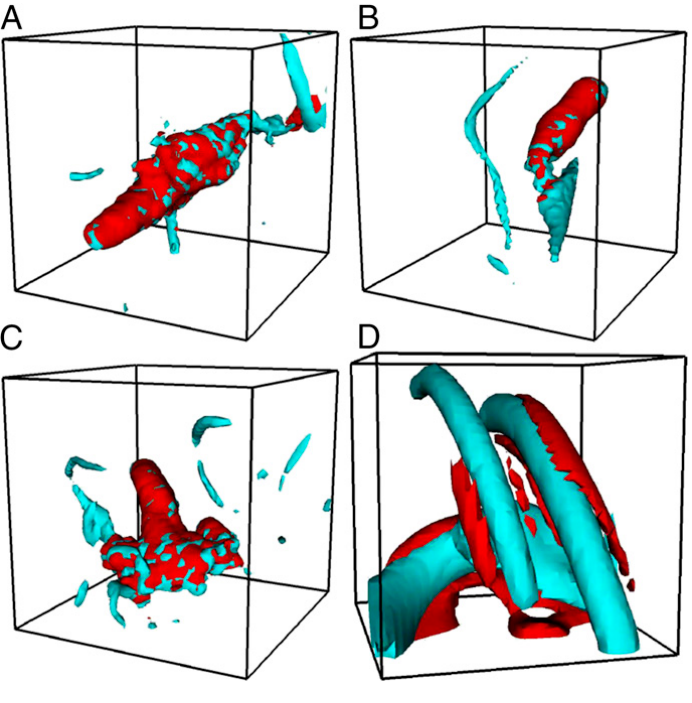
\includegraphics[width=30pc]{gfx/Yeung_chunky_vortices.png}
\caption{Color contours based on: (A-C) three instantaneous snapshots from the $8,192^3$ simulation at $R_\lambda \approx 1,300$, contrasted with data from (D) $2,048^3$ simulation at $R_\lambda \approx 400$. The contour thresholds used were 300 for data at $R_\lambda \approx 1,300$ and 70 for data at $R_\lambda \approx 400$. The subcubes are $51^3$ in extent in A-C and $31^3$ in D. Reprinted from \citet{Yeung2015}.}
\label{fig:ch1_03}
\end{figure*}

The reports mentioned above, as well as other studies, mean that we do not really know what to expect in turbulence with even higher $Re$. The values achieved in the laboratory and simulations, although becoming higher and higher, are still far from those found in atmospheric turbulence. This is one of the reasons why we are not sure whether the results of the intermittency and structure research can be applied to the atmosphere. In the next paragraph I try to elaborate on this problem.
 
\subsubsection{Atmospheric turbulence}
Turbulence in atmosphere, especially in clouds, influence many important processes: it governs entrainment and mixing, impacts cloud droplet evolution and interacts with large-scale cloud dynamics \citep{Bodenschatz2010}. In-situ measurements of cloud-related turbulence are scarce and there are several reasons for that. Obviously it is not possible to have any control over the meteorological conditions. Observations made with research aircrafts are one-dimensional, prone to aerodynamic errors and of relatively low resolution due to  large true airspeed. Measurements at mountain research stations are biased by orographic boundary conditions. Experimental equipment used must be resistant to hard meteorological conditions and large speeds/vibrations etc. Last but not least, field campaigns in atmospheric research are much more expensive then laboratory experiments. Despite these discouraging factors, the effort put into atmospheric turbulence measurement should pay off: after all, at our fingertips we have turbulence with the highest $Re$ on Earth and a huge range of scales spanned between the smallest and largest eddies of turbulence, from parts of millimeters to kilometers. Little experimental evidence and complementary Direct Numerical Simulation (DNS) studies focused on atmospheric turbulence are summarised below.\\
Turbulence in the atmosphere is hard to analyse because of the presence of large scale anisotropies, inhomogeneity of turbulence field and nonstationary effects due to stratification, presence of liquid water and water vapor, aerosols of all kinds, sun heating, Coriolis force etc \ref{Wyngaard2010}. Part of my own research concentrated on some of these factors. On the basis of relatively large data set collected in the Physics of the Stratocumulus Top (POST) campaign by in-flight measurements, we tried to characterize turbulence and passive scalars properties in marine boundary layer clouds \citep{Jen-LaPlante2016, Ma2017}. The investigation revealed complex structure of Sc cloud and its surrounding, showing turbulence inhomogeneity at the range of scales reaching depth of inertial range. The transport of energy and momentum between these inhomogeneous spatial regions, called layers (TISL, CTMSL and CTL mentioned earlier in the text), is nonuniform, as well as the scaling behaviour of temperature and so called \emph{liquid water content} (LWC, mass of the water in a cloud in a specified amount of dry air). But what is most distinctive in the results is strong anisotropy of turbulent motions at many scales \citep{Pedersen2018}. Vertical fluctuations seem to be damped by static stability and horizontal fluctuations to be enhanced by large scale shear. This topic needs to be adressed more carefully, especially since some studies indicate that large scale anisotropy can be transmitted to small scales and be related with small-scale intermittency \citep{Warhaft2002} or can totally change turbulence structure by appearing as large-scale intermittency\citep{Takahashi2018}. The paradox however is that in all the turbulent studies in order to calculate turbulence properties such as $TKE$, $\epsilon$, $\eta$, assumptions of isotropy, homogeneity and stationarity of small scales of turbulence are taken. What is particularly interesting, is that dissipation range is usually still not resolved in the in-situ atmospheric measurements, but $\epsilon$ estimation attracts particular attention. Its value is smaller by a few orders of magnitude then typically observed in the laboratory \citep{Siebert2009, Jen-LaPlante2016}. Some effort is put into improving $\epsilon$ estimation by accounting for low-resolution of the measurements (see Fig. \ref{fig:ch1_04} from \citet{Waclawczyk2017}) or stratification and shear influence \citep{Zilitinkevich2019}. \\

\begin{figure*}
\centering
\noindent 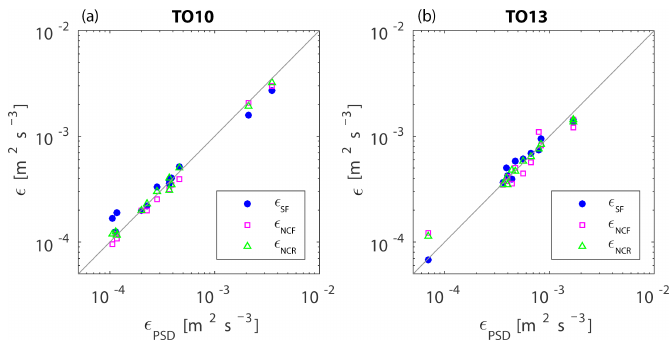
\includegraphics[width=30pc]{gfx/epsilon_methods_POST.png}
\caption{Dissipation rate of the kinetic energy estimated from the structure function method $\epsilon_{SF}$, zero crossings of successively filtered signals $\epsilon_{NCF}$ and zero crossings of signals with recovered part of the spectrum $\epsilon_{NCR}$ as a function of $\epsilon_{PSD}$ (from the power spectra
method). Each point represents an estimate from a single horizontal segment of flight in the atmospheric boundary layer. (a) POST flight TO10 (b) POST flight TO 13. Reprinted from \citet{Waclawczyk2017}. Description of estimation methods available in the source paper.}
\label{fig:ch1_04}
\end{figure*}
In conclusion, turbulence in the atmosphere, especially in the clouds, has properties that differ from turbulence created in the laboratory conditions. The language used to describe atmospheric turbulence is based on assumptions that are not fulfilled. Therefore, there is a need for research on its basic aspects, its structure and dynamics. This thesis by dealing with a simplistic model of cloud droplets moving in turbulence and trying to understand unique experimental evidence, offers a small contribution to the understading of these basics. Next paragraph focuses on the great challange which is efficient description of particle motion in the specific flow.


%----------------------------------------------------------------------------------------
\subsection{Single particle motion in the flow}

In order to study the dynamics of particles advected by turbulent flow, one needs to have a simple formulation of the equations of motion of the advected particles. The problem is that particles of particular interest, namely cloud droplets, are finite-size, which means they are actually extended objects with their own boundaries. The rigorous way to analyse their dynamics would involve solving the Navier–Stokes equation for moving boundaries. The partial differential equations resulting from this approach are very difficult to solve and analyse. In many approximate derivations, the common concept that arises from the mathematical development is that of undisturbed fluid velocity, i.e. the velocity that the fluid would have had at the absence of the particle. In this way the flow is separated into the flow field as it would have been without particles, and the disturbance field. Widely used and very popular is the approximate differential equation for the motion of small spherical particle in the  flow that was written down by Maxey and Riley in 1983 \citep{Maxey1983}:
\marginpar{Maxey-Riley equation}
\begin{align}
\vec{v}=\dot{\vec{r}},\\
m_p \dot{\vec{v}}=\overbrace{m_f \frac{\mathrm{D \vec{u}}}{\mathrm{D}t}}^{(1)} -\overbrace{ \frac{1}{2} m_f \left[\dot{\vec{v}}- \frac{\mathrm{D }}{\mathrm{D}t} \left( \vec{u}+\frac{1}{10} R^2 \nabla^2 \vec{u}\right) \right]}^{(2)} -\overbrace{6 \pi \mu R  \vec{q}(t)}^{(3)}\\
\nonumber +\underbrace{\left(m_p-m_f\right)\vec{g}}_{(4)} -\underbrace{6 \pi \mu R^2  \int_{0}^{t} \mathrm{d}\tau \frac{\mathrm{d}\vec{q}(\tau)}{\mathrm{d}\tau} (\pi \nu \left(t-\tau\right))^{-\frac{1}{2}}}_{(5)}
\label{ch1:eq02}
\end{align}
where:
\begin{description}
\item $\vec{r}(t)$ - position of the particle at time t,
\item $\vec{v}(t)$ - velocity of the particle,
\item $\vec{u}(r(t),t)$ - undisturbed fluid velocity at the location of the particle,
\item $\vec{q}(t)=\vec{v}(t)-\vec{u}(\vec{r}(t),t)-R^2\nabla^2\vec{u}(\vec{r}(t),t)/6$ - particle-fluid velocity difference with correcting factor,
\item $R$ - particle radius,
\item $m_p$ - particle mass,
\item $m_f$ - mass of the fluid displaced by the particle,
\item $\rho_f$ - fluid density,
\item $\mu$ - fluid dynamic viscosity, 
\item $\nu$ - fluid kinematic viscosity,
\item $\vec{g}$ - gravitational acceleration,
\end{description}
and the derivatives:
\begin{description}
\item $\frac{\mathrm{D}}{\mathrm{D}t}=\frac{\mathrm{\partial}}{\mathrm{\partial}t}+\vec{u} \cdot \nabla$ - the material derivative (along fluid path), 
\item $\frac{\mathrm{d}}{\mathrm{d}t}=\frac{\mathrm{\partial}}{\mathrm{\partial}t}+\vec{v} \cdot \nabla$ - total derivative along particle trajectory.
\end{description}

The \emph{Maxey-Riley equation} (M-R) consist of a few terms which has the following physical interpretation.
\begin{description}
\item (1) - force exerted on the particle by the undisturbed fluid element in position $\vec{r}(t)$ at time $t$.
\item (2) - \emph{added-mass effect}, accounts for the fact that when the particle accelerates relative to the fluid, it displaces a certain amount of fluid with it.
\item (3) - Stokes viscous drag.
\item (4) - buoyancy force.
\item (5) - Basset history term, arises from the fact, that the vorticity diffuses away from the particle due to viscosity.
\end{description}
The terms involving the factor $R^2 \nabla^2 \vec{u}$ (in (2), (3), (5)) are the \emph{Faxén corrections}, and they account for the spatial variation of the flow field across the particle. Simulations have shown  however \citep{Calzavarini2012} that the Faxen correction becomes significant only for particles with diameter of several times the dissipative (Kolmogorov) length scale of the flow (unlike cloud droplets). M-R equation is generally valid for small particles at low particle Reynolds numbers $Re_p$. This Reynolds number is calculated by using the relative velocity between particle and neighbouring fluid as the velocity scale: 
\begin{equation}
Re_p = R|\vec{v} - \vec{u}|/\nu.
\label{def:Rep}
\end{equation}
This implies that for M-R eq. to be a valid approximation, the initial velocity difference between particle and fluid must be small. Another condition is that the shear Reynolds number $Re_{\zeta} = R^2 \zeta/\nu<<1$, where $\Gamma$ is the typical velocity gradient in the flow, must be small.\\
The M-R equation can be simplified with the adoption of appropriate assumptions. We call a particle:
\marginpar{small, heavy, inertial, sedimenting particle}
\begin{itemize}
\item \emph{heavy} when its density is significantly larger than fluid density $\rho_f<<\rho_p$,
\item \emph{small} when its radius is significantly smaller then smallest fluid spatial scale $R<<l_f$,
\item \emph{sedimenting} when its subject to gravity force
\item \emph{inertial} when its response time $\tau_p$ (to be defined) is larger then smallest fluid time scale $\tau_p>\tau_f$
\end{itemize}
When the particle follow these assumptions then the M-R eq. is of the form:
\begin{align}
\vec{v}=\dot{\vec{r}},\\
\dot{\vec{v}}=\tau_p^{-1}\left(\vec{u}(\vec{r},t) -\vec{v}(t)\right)+\vec{g}-(5)/m_p
\label{ch1:eq03}
\end{align}
where $\tau_p=2 \rho_p R^2/9\mu$ is the particle inertial response time and $(5)$ stands for the Basset history term. In this thesis droplet trajectories are calculated with the use of the approximated M-R equation- Eq.\ref{ch1:eq03} without history term $(5)$:
\begin{equation}
\vec{v}=\dot{\vec{r}},\\
\dot{\vec{v}}=\tau_p^{-1}\left(\vec{u}(\vec{r},t) -\vec{v}(t)\right)+\vec{g}
\label{ch1:eq04}
\end{equation}
The history term is ommitted in this thesis due to its huge cost in numerical simulations. In the next section I discuss the applicability of certain M-R equation terms for cloud droplets in the vortex model.(??? czy na pewno dyskutuje gdzies ???)\\ 
\marginpar{tracers}
The other important class of particles are so called \emph{tracers}: their density is equal to fluid density and they follow the flow exactly, unlike the inertial particles, which detach from the flow. The main difference between dynamics of tracer and inertial particles is that volume in phase space of tracers is conserved, whereas that of inertial particles shrinks. Tracers serve as benchmark particles in clustering studies.\\
Particle motion research require the use of some nondimensional numbers, which describe ratio of forces working on a particle. These are Stokes number $St$, sedimentation parameter $Sv$ and Froude number $Fr$. \marginpar{Stokes number}$St$ characterizes the inertia of the particle, while it is the ratio of the particle response time to fluid characteristic timescale. 
\begin{equation}
\nonumber St \equiv \tau_p/\tau_f
\label{def:St}
\end{equation}
\marginpar{sedimentaion parameter}$S_v$ is nondimensional settling velocity (the ratio of terminal velocity $v_g$ to the fluid characteristic velocity $v_f$). 
\begin{equation}
\nonumber Sv \equiv v_g/v_f
\label{def:Sv}
\end{equation}
The ratio of Stokes number to the sedimentation parameter is Froude number $Fr$. \marginpar{Froude number}It expresses the same time the ratio of particle response time $\tau_p$ to the residence time of the particle in a Kolmogorov eddy.
\begin{equation}
\nonumber Fr \equiv St/Sv
\label{def:Fr}
\end{equation}
$Fr$ is considered a measure of the influence of gravitational force on the droplet motion. In the limit of a large Froude number, gravity is seen as negligible. \\
Thus equipped with the tools of single particle motion description, one may proceed to the complex issue of particle motion in turbulent flow.

%----------------------------------------------------------------------------------------
\subsection{Particle motion in turbulent environment}

Many efforts were made to understand the dynamics of multiphase turbulent flows. Despite that few definite conclusions can be drawn. The development of Lagrangian techniques ("following" a particle motion in the fluid) in recent years has shed some new light on the relation between particle motion and fluid motion. However we are still far from creating a thorough theory describing how (and why) particles behave in turbulent flow. The dynamics and kinematics of fluid tracers themselves are in fact the subject of current discussion \citep{Biferale2005,Arneodo2008, Toschi2009,Scatamacchia2012,Dhariwal2018}. In case of inertial, heavy particles there are more questions then answers. Just to start, no comprehensive investigation of the consequences of all simplifications usually made in inertial particle motion studies has been made yet \citep{Bourgoin2014}. Some studies try to answer what is the accuracy of Stokes drag model (term $(3)$ in Eq. \ref{ch1:eq02}) when comes to particle relative velocities (see \citet{Dou2018} or \citet{Saw2014} concerning water droplets in the air) or if Basset-history force,  hydrodynamic interactions or turbulence small-scale anisotropy play any important role. Others consider the impact of Reynolds number as well as gravity\citep{Ireland2016a, Ireland2016b}. The issues raised above may substantially affect validity of the results regarding particle statistics in turbulence such as spatial distribution, collision probability, condensational growth or sedimentation velocity \citep{Chen2018}. These statistics are especially important in cloud physics, as they determine rain formation process and cloud radiative properties. Better understanding how turbulence influences them by interaction with cloud droplets would lead to more precise characterization of cloud evolution\citep{Bodenschatz2010}. Until now there has been a lot of theoretical and numerical research done but there is no agreement what are the key turbulent processes in this evoulution (for reviews see \citet{Vaillancourt2000, Shaw2003, Devenish2012, Grabowski2013, Pumir2016, Saito2018}). There are however some suggestions that the key processes are connected to the facts that even slight change of local droplet concentration (clustering, see next paragraph) or violent local turbulent events may influence cloud droplet growth significantly \citep{Kostinski2005, Bec2016, Madival2019}. Experimental studies in the atmosphere \citep{Chaumat2001, Pinsky2001, Kostinski2001, Shaw2002, Knyazikhin2005, Marshak2005, Lehmann2007, Glienke2017} and in the laboratory \citep{Jaczewski2005, Warhaft2008} for long time have been inconclusive about the occurrence of clustering of cloud droplets on small-scales. Recently \citet{Larsen2018} have finally revealed that there is statisticaly significant and unambiguous evidence of weak clustering on scales between about 1 and 5~mm (around 1$\eta$ and 5$\eta$) for polydisperse set of cloud droplets larger then $10\mu m$ in weakly turbulent clouds. This thesis focus on the turbulence influence on droplet spatial distribution (clustering) in the context of cloud evolution. Next paragraph introduces this problem broadly.\\
 \marginpar{clustering}
Clustering is the central term when talking about statistical change in spatial distribution. It occurs when particle distribution deviates from random distribution, in our case due to the interaction of inertial particles with turbulent flow. There have been numerous studies on particle clustering motivated by industrial, geophysical or astrophysical apllications. Most of the numerical and theoretical research focus on monodisperse and non-sedimenting particles in homogeneous, isotropic turbulence (HIT), and numerical simulations are conducted in Taylor microscale Reynolds number $Re_{\lambda}$ which is a few order of magnitudes smaller than in the atmosphere. Thus  application of such research to cloud droplet clustering is limited without further experimental investigation of polydispersity or gravity impact, matter of $Re_{\lambda}$ increase or turbulence anisotropy/inhomogeneity influence. However, in order to properly address the complex problem, I will first review what has been achieved in a reduced problem.\\
Monodisperse, heavy inertial and non-sedimenting particle clustering in HIT in theory may be divided into three regimes: small-scale clustering, preferential sampling and short-time clustering due to caustics (or sling effect) - this division and review is available in \citet{Gustavsson2016}. \emph{Small-scale clustering} occurs on scales smaller than correlation length of the flow which in realistic turbulence is spatial Kolmogorov scale $\eta$ representing the size of dissipative eddies. \marginpar{small-scale clustering}Small-scale clustering demonstrates self-similarity (clustering properties are independent of scale) and is often described with statistical and dynamical methods developed for multifractals \citep{Falkovich2003, Bec2005, Bec2006b, Bec2007, Bragg2014}. Yet analytical calculations concerning small-scales are possible only for substantially simplified statistical models of turbulence. The hope is that the only experimental work treating about dissipation-scale clustering, that was conducted by 1D measurements on polydisperse particles in low $Re$, large $\epsilon$ turbulence, is in qualitative agreement with the theory \citep{Saw2008}.\\
\marginpar{Preferential concentration/sampling} \emph{Preferential sampling} or preferential concentration appears at inertial scales of turbulence when particles sample only regions of the flow that posses specific features.  Most frequently cited approach to preferential concentration, generated for particles in small $St$ expansion, is a so called “Maxey centrifuge” mechanism \citep{Maxey1987}. It claims that small heavy particles gather in straining regions of the flow and are centrifuged out of vortical regions. This  concept was further developed in many numerical and theoretical studies (see for example \citet{Sigurgeirsson2002,Cencini2006}) and confirmed experimentally (for latest see \citet{Bhatnagar2018}). Alternative description formulated on the basis of DNS simulation results is \emph{sweep-stick mechanism} \citep{Goto2008,Coleman2009}, which states that particles stick to regions of low fluid acceleration as they are swept through the flow.\marginpar{sweep-stick mechanism} There were some other theoretical and numerical views using statistical methods proposed as well, see for example \citet{Falkovich2002, Bec2007, Hartlep2017}. \citet{Bragg2015a} claim that actually physical mechanisms of clustering at dissipative and inertial scales in HIT are the same and they provide the fundamental explanation for this fact. The key parameter used in their analysis is the \emph{local Stokes number} $St_l$ defined for an arbitrary spatial scale $ \eta << l << L$. \marginpar{local Stokes number}It expresses the ratio of particle response time to $\tau_l= \langle \epsilon\rangle^{-1/3} l^{2/3}$ - the eddy of size $l$ turnover time. For any separation $l<<L$, the clustering mechanism for $St_l<<1$ is related to preferential sampling of the fluid velocity gradient tensor $\nabla \vec{u}$ coarse-grained at scale $\approx l$, which is associated with centrifging out of eddies at that scale. They point as well the that this mechanism is in close relationship to sweep stick mechanism in the inertial range. For $St_l \geq O(1)$ a nonlocal mechanism contributes to the clustering process. One can take a lesson that when dealing with clustering, it is important to define the nondimensional parameters suited to the model used.\\
The other, quite new approach to clustering analysis puts in the center of attention the concept of coherent clusters of particles: their formation time, size, the local concentration in the cluster as well as their dependence on $Re_{\lambda}$, $St$, $Sv$, $Fr$. \citet{Baker2017, Momenifar2019} on the basis of DNS analysis claim that particles in the cluster exhibit significantly higher degree of spatial organization and local acumulation, that their sedimentation velocity is higher that outside the cluster and that clusters align themselves with the local vorticity vector. Most of the  experiments concerning preferential concentration focus on cluster and void analysis as well, using the technique of Voronoi triangulation \citep{Monchaux2010,Monchaux2012, Obligado2014, Sumbekova2017, Manish2018}. Some of the research described here lead to the suggestions that turbulence intermittency and cluster/void formation are linked.\\
 Clustering by \emph{caustics} is the least known mechanism of the most complicated structure. The mathematical definition is that they are singularities in particle dynamics i.e. particles of totally different velocities meet in the same space point (see review in \citet{Gustavsson2016}). More picturesque formulation of the same mechanism is the sling effect: particle is expelled out of the vortex as if it was shot with a sling. They were observed in numerical simulations \citep{Marcu1995, Falkovich2007, Bec2011, Bewley2013}. Very recent works of \citet{Ravichandran2015, Deepu2017} connect them directly to strong enhancement in particle collision probability.
\\
Recent developement in massive numerical computations made it possible to take into account other forces acting on the particle like computationally demanding Basset history force \citep{Olivieri2014} or hydrodynamical interaction \citep{Monchaux2017, Yavuz2018} (so called "two-way coupling") and check if they impact clustering processes. The results of this work are not yet conclusive, but they lead to understanding that these forces may be of great importance. Meanwhile, sedimentation influence on clustering and vice-versa has already been explored in DNS and theory in more detail \citep{Wang2006, Ayala2008, Woittiez2009, Dejoan2013, Gustavsson2014, Bec2014, Park2014, Bragg2015b, Rosa2016, Ireland2016b, Rosa_Pozorski2017,Baker2017, Tom2019, Momenifar2019}. Nevertheless the role of gravity in clustering remains an open field. For now, it seems that gravity weakens the clustering of small particles $St<1$ and increases of large particles $St>1$.
\\
The advances in studies on clustering of monodispersed particles in HIT has been summarized above. The matter is far more complicated when it comes to the collection of polydispersed particles. Recognizing the influence of polydispersity on clustering is especially important when interpreting experiments with small particles and veryfing a theory on experimental basis. Natural sets of particles (like cloud droplets), but also those produced in the laboratory, usually are biased by unavoidable polydispersity. Many of the DNS and laboratory experiments cited here as monodispersed particle studies have sections dedicated to polydispersity influence. First, but still unsolved problem in dealing with polydisperse particles is choosing statistical variables that can represent the size distribution with respect to clustering processes. There were many propositions, from mean arithmetic Stokes number, to various volume, surface or particle number weighted means. Secondly, the problem is the very way of describing clustering, which would capture its complexity. Some try to define a single measure of segregation \citep{Calzavarini2008}, other analyze collective radial distribution function (RDF) \citep{Saw2012a, Saw2012b} as well as cluster sizes, structure and motion \citep{Lian2013, Lian2019}. \citet{Minier2016} reviews available statistical description methods of polydisperse, multiphase turbulent flows. Generally the scarce research agrees on a few topics. Even mild polydispersity (like $\Delta St > \langle St \rangle/5$ in \citet{Saw2012a, Saw2012b}) reduces overall clustering. The lengthscale of droplet clusters falls into ranges 10-30, 20-30, 40-50 $\eta$ (depends on the study), so in dissipation range. The lifetime is longer then $\tau_{\eta}$ and that more than just particle mean $\langle St \rangle$ is needed to statistically discribe clustering. There is no agreement if there is dependence on $Re_{\lambda}$, turbulence intensity or shape of size distribution, or if cluster sizes depend on $St$.\\
From the above summary of research on clustering we can conclude that the basic mechanisms have still not been understood enough to grasp its impact on cloud evolution. \emph{Tu jeszcze zdanie o wnioskach z powyzszego, do ktorych odwolujemy sie przy analizie dziur.} Next I follow the concept that structures connected to turbulence intermittency may play a significant role in particle spatial distribution change. However fully resolved simulations of NSE for atmospheric-like turbulence is beyond computational reach, hence the need to examine reduced models.

\subsection{Vortex structures versus cloud droplet clustering}

The concept of the paper by \citet{Kostinski2005} is that the factor of-10 acceleration in the growth of the “lucky” droplets (the fastest one-in-a-million) combined with traditional turbulent cascade ideas is enough to explain the size-gap problem in cloud droplet growth theory. This gap, called condensation-coalescence bottleneck as well, is a lack of understanding the processes bringing in around 15~min  cloud droplets, that grew by condensation to around 20~$\mu m$ in radius, to 40~$\mu m$, for which size gravitational collisions become effective growth process. Although the \citet{Kostinski2005} paper did not explain how to get such a fast growing lucky droplet, it gave the lesson that even very rare local events may have great impact on global state of a cloud. \citet{Bec2016} showed in statistical analysis of DNS that there is precise connection between the intermittent nature of the carrier turbulent flow and the accelerated growth of particles by increased collisions. However one may miss important information when paying attention to global statistics only, for example where and how this collisions occur. For this reason, the researchers studying the distribution and collisions of particles in the flow, became interested in the trend of searching for coherent structures in turbulence that can influence this processes \citep{Davila2001, Bec2006a, Biferale2016, Bhatnagar2016, Perrin2016}.\\
It was mentioned before, that intense vortex structres (or vortex tubes) probably play important role in turbulence intermittency and hence may have particular impact on dynamics of heavy inertial particles. Previous efforts to study this dynamics in vortices were made by simulating droplet trajectories in a prescribed velocity field for several simple single-vortex models. Such research for the simplest model of a line vortex with stretching was conducted by \citet{Markowicz2000} with limitation to horizontally oriented vortices. Some specific features of droplet trajectories for monodisperse droplets in another model, a Burgers vortex with stretching, were examined in 2D by \citet{Marcu1995} for arbitrary alignment with respect to gravity and by \citet{Hill2005} for horizontal alignment together with collisions. \citet{Ravichandran2014} studied the behaviour of particles near fixed points, with no gravity, between two like-signed vortices. \citet{Ravichandran2015} analysed lagrangian density around the particle in 2D point vortex, gaussian vortex and collection of point vortices (no gravity), especially with respect to caustics formation. \citep{Deepu2017} used this analysis for polydisperse droplets to show growth of particles by increased collisions around single vortex.  \citet{Picardo2019} in the DNS of turbulent flow (without gravity) indicate the regions that are possibly responsible for enhanced collision probability - vortex-strain worm-rolls - and claim that particles in intense vortex tubes are rapidly ejected into strong straining sheets. On the whole, interest in the topic of the vortices role in particle clustering and collisions has been considerable in recent years. My research was part of this trend and surely filled in one of the gaps. Namely, in my investigation I took into account the 3D motion of a particle under gravity force as well as described the collective motion of polydispersed particles in a vortex as a proxy of droplets in a real cloud turbulence.\\

\section{Research problem statement}
Generally the objective of this research is to show that in cloud turbulence, presence of a long-lasting, violent vortical structure is probable and it can cause strong local clustering and segregation of cloud droplets. There are several research ideas behind it.
I assume that the motion of a single sedimenting particle in the Burgers vortex model with stretching can be described by means of the formalism of dynamical systems. For some sets of vortex and particle parameters the motion of a particle in two dimensions is determined by different types of attractors and cannot be reduced to Maxey centrifuge mechanism. First hypothesis is that these 2D attractors are crucial in 3D particle motion as well. Second hypothesis states that there is significant clustering of particles near the vortex and in polydispersed systems it leads to a strong size segregation.\\
Another goal of this thesis is to describe in detail first-of-a-kind observations of relatively large heterogeneities in the form of near-circular "voids" in atmospheric clouds \citep{Xu2012}. This work attempts to answer the question whether these structures can be explained solely by the presence of a strong vortex in the field of cloud droplets when moddeled according to the above assumptions. Complementary study identifies the conditions under which the void phenomenon in the selected model is created and indicates the potential high impact of imaging technique on voids observation. To the best of author's knowledge, the most novel aspects of this work are complexity of the model chosen for analysis and its apllication to explain unique in-situ experiment results.\\
Verification of hypotheses set in this thesis is conducted with the use of simplified model. Particles are small, sedimenting, heavy, inertial and noninteracting with each other, a vortex tube model is Burgers vortex with stretching. The only forces working on particle is Stokes drag and gravity and there is no hydrodynamical interaction between particle and the flow. On the basis of the numerous literature sources cited above I assume that a single, steady, stationary vortex is a good proxy for a rare vortical event in high $Re$ turbulent flow as to inspect particle motion inside the structure. The Burgers vortex is a reasonable approximation of such a localised in time and space single vortex in the flow. Collisions of particles are not taken into account to extract vortex influence on spatial distribution of particles only.\\
As far as the observations are concerned, it is assumed that the measurement results from mountain-top observatory were not disturbed by the presence of boundaries. Further in the text there is discussion of this assuption. What is most important, however, is that I analyzed one and only case of cloud "voids" ever recorded. These observations were the only one of its kind and have not been repeated to this day. During my doctoral studies I was preparing a measurement campaign to confirm these results, with the use of a newly designed device. The prepared equipment, operating well in laboratory conditions, did not comply with harsh conditions present in a cloud at the mountain observatory. The experimental difficulties accompanying the registration of a single droplet in a real cloud are described in the following chapters.\\
Due to numerical power limitations, the Basset history force is not included in particle motion simulations. Its role in particle motion in turbulence is a subject of most recent, separate studies. Another consequence of numerical power limitations is that simulations do not reproduce the particle number concentrations corresponding to cloud values.\\


%M.in. stosowalnosc rownania M-R poruszyc?.Coś o Re_p?

%https://books.google.pl/books?id=5SW7BQAAQBAJ&pg=PA53&lpg=PA53&dq=maxey+and+riley+equation+assumptions+approximation&source=bl&ots=jj3CG0Cj4w&sig=ACfU3U1_uEL-TcuvpYZgUf5yqVi_F3yKxA&hl=pl&sa=X&ved=2ahUKEwiJs_W0rajkAhWIqIsKHQKACK4Q6AEwBXoECAkQAQ#v=onepage&q=maxey%20and%20riley%20equation%20assumptions%20approximation&f=false
%http://www.iact.ugr-csic.es/personal/julyan_cartwright/PDFs/79_2010_Springer.pdf
%https://doi.org/10.1016/j.ijmultiphaseflow.2016.10.003
%https://doi.org/10.1017/jfm.2015.551

%Type of assumption most commonly stated explicitly is one that is limited in its nature and serves to hold the size or scope of an investigation within its prescribed boundaries (puts parameters around the study).
%Usually made when the argument rests on a priori reasoning, but can be made on basis of present knowledge on research which is as yet incomplete (Specific qualifications must be made in the conclusions of the research report in which assumptions are made.)
%Protects researcher, e.g., keeps someone from saying, "Oh, I thought you were studying XYZ, too.”


\end{document}
